\ProvidesFile{ch3.tex}[Chapter4]

\chapter{Quantum enhanced localization with a single photon avalanche diode array}
\ix{physics//Physics appendix}

\section{Introduction}

\subsection{A brief introduction to quantum optics}

Experimental techniques have surfaced which take advantage of the quantum nature of light to enhance imaging methods. The advent of very fast and sensitive detectors allows us to measure EM fields at a timescale where quantum effects can be seen. We often speak of concepts such as photon counting or photon statistics, and it is prudent to define what a photon really is and how it be measured with this technology. Therefore, it is necessary to define a very basic formulation of the quantization of the electromagnetic field. 

We start by stating the major results of quantizing the EM field at a single point in space, which could be a point detector element, for example. Quantizing the field at a single point in space simplifies the problem to focusing only on time dependence where spatial heterogeneity of the field can be ignored. We express the time-dependent field as a sum of harmonic oscillators using a Fourier series expansion. We consider an oscillation $E(t)$ that can only exist in one dimension, or a single polarization, making the field effectively a scalar one. This decomposition represents the field in terms of an infinite number of modes indexed by $k$ with frequency $\omega_{k}$ i.e., $E(t) = \sum_{k=1}^\infty c_{k}e^{-i\omega_{n} t}$. In order to quantize the field, each mode is treated as a quantum harmonic oscillator. As such, the Hamiltonian for one particular mode is that of a quantum harmonic oscillator which has energy eigenvalues $E_{k} = \hbar\omega_{k}(\hat{n} + \frac{1}{2})$. The operator $\hat{n}=\hat{a}^{\dagger}\hat{a}$ is the number operator such that $\hat{n}\ket{\psi} = n\ket{\psi}$ where $n$ is the number of energy quanta in that particular mode. The value of $n$ represents the number of energy quanta present in the field, each quanta being called a photon. Since there are potentially infinitely many modes, the wavefunction at this point is then $\ket{\psi} = \ket{n_{1},n_{2},...}$ where $n_1$ is the number of photons in the first mode, $n_2$ is the number of photons in the second mode, and so on. The number operator for the $n$-th mode is $\hat{n}_k\ket{\psi} = n_{k}\ket{\psi}$. 

We also define $\hat{a}_n$ and $\hat{a}_n^\dagger$ as the respective annihilation and creation operators for the $n$-th mode. These operators satisfy the commutation relations $[\hat{a}_k, \hat{a}_k'^\dagger] = \delta_{kk'}$ and $[\hat{a}_k, \hat{a}_k'] = [\hat{a}_k^\dagger, \hat{a}_k^\dagger] = 0$. The action of the annihilation and creation operators on the joint number states is:

\begin{equation*}
\hat{a}_k \ket{n_1, n_2, ...} = n_k \ket{n_1, n_2, ...} \;\;
\hat{a}_k^\dagger \ket{n_1, n_2, ...} = (n+1) \ket{n_1, n_2, ...}
\end{equation*}

\subsection{Photon statistics}

At this point in space, we can define any $\ket{\psi}$ that we like in this framework. However, there are certain interesting states which have special properties, such as the coherent state. Coherent states are a special class of states that resemble classical states of the EM field. Qualitatively, at a point, they would give rise to a coherent sinusoidal behavior of the field. Suppose we have a single mode field in a state $\ket{m}$. A coherent state $\ket{\alpha}$ is defined as the eigenstate of the annihilation operator $\hat{a}$:

\begin{equation*}
\hat{a} \ket{\alpha} = \alpha \ket{\alpha}
\end{equation*}

where $\alpha$ is a complex number. The coherent states are given by:

\begin{equation*}
\ket{\alpha} = e^{-\frac{\lvert\alpha\lvert^2}{2}} \sum_{m=0}^\infty \frac{\alpha^m}{m!} \ket{m}
\end{equation*}

It turns out that if we measure a number of photons (intensity) in this state, we would find that the number of photons has Poisson statistics. To see this, we calculate the probability $P(m)$ of finding $m$ photons in a coherent state $\ket{\alpha}$:

\begin{equation*}
P(m) = \lvert \bra{m} \ket{\alpha} \lvert^2 = \lvert e^{-\frac{\lvert\alpha\lvert^2}{2}} \frac{\alpha^m}{m!} \lvert^2 = e^{-\lvert\alpha\lvert^2} \frac{\lvert\alpha\lvert^{2m}}{m!}
\end{equation*}

This is simply the Poisson distribution with mean $\langle \hat{n}_n \rangle = \lvert\alpha\lvert^2$. The variance of the photon number distribution in a coherent state is also $\lvert\alpha\lvert^2$, characteristic of Poisson statistics, where the mean and variance are equal. 

In contrast, single photon states e..g, $\ket{1}$ do not necessarily follow Poisson statistics. This state could be prepared by an isolated single photon source such as a fluorescent dye molecule which can produce only a single photon at at time. This phenomenon is referred to as \emph{fluorescence antibunching} where photons tend to be detected as isolated events rather than in bursts or bunches. Note that for such a single photon source the single-mode field can be in state $\ket{1}$ but not state $\ket{2}$ at any given time. If more single photon sources are present states beyond $\ket{1}$ are achievable. This has led to the introduction of binomial states of the quantized field.


Far-field optical microscopy is fundamentally limited by diffraction, with the maximum attainable resolution being limited to approximately half the wavelength of light. Several schemes to beat the diffraction limit have been developed in recent years. Many of these schemes utilize the concept of precise localization of isolated fluorescent emitters which blink over a time series of frames \parencite{Rust2006,Betzig2006}. An inherent problem with such methods is the requirement that fluorescent emitters be isolated, slowing down the acquisition of super-resolved images. To address this, we leverage the fact that many fluorophores are intrinsically single photon sources and exhibit fluorescence antibunching. This property can constrain the number of active fluorescent emitters in a region of interest (ROI) and can potentially enable localization in non-sparse scenes \parencite{Ta2010,Israel2017}. 

\begin{figure*}[t]
\centering
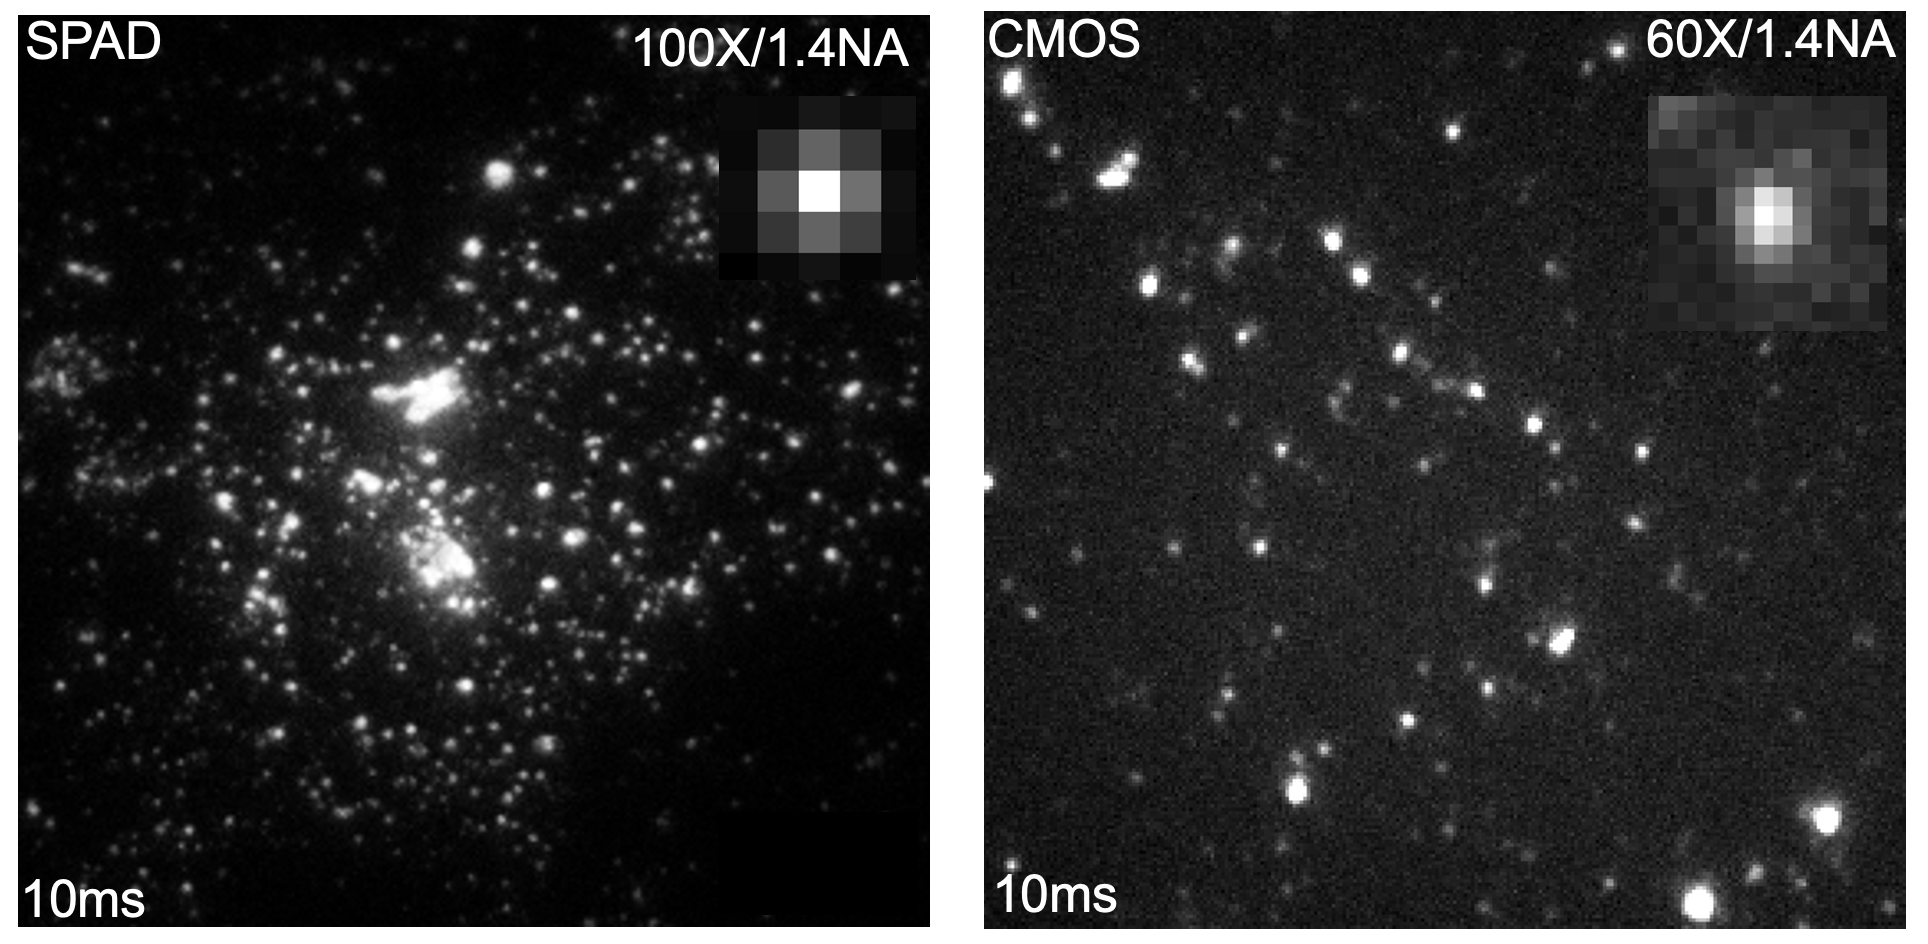
\includegraphics[width=14cm]{/Users/cwseitz/git/cwseitz.github.io/docs/phd/spad/spad/media/SPADvCMOS.png}
\caption{Comparison of quantum dot images between CMOS and SPAD cameras. (left) SPAD image of Qdot655 images using a 100X/1.4NA oil-immersion objective (Nikon) and a 10ms exposure time. (right) CMOS image of Qdot655 using a 60X/1.4NA oil-immersion objective (Olympus) and a 10ms exposure time.}
\end{figure*}    

Molecular counting with fluorescence antibunching has a fairly simple motivation: coincidence of photons at multiple detector elements during high speed imaging provides evidence for the number of single photon sources present in the imaged region. Combining the ideas of conventional super-resolution approaches with photon statistics may prove to be a powerful set of methods for bioimaging. SPAD cameras achieve orders of magnitude higher temporal resolutions than standard CMOS cameras, single photon sensitivity, and dark count rates less than 25cps. Furthermore, the reduced readout noise and large fill-factor of recently commercialized SPAD arrays suggests their use for single molecule localization with reduced localization uncertainty. Localization uncertainty, typically the root mean square error (RMSE) of a maximum likelihood or similar statistical estimator, is bounded from below by the inverse of the Fisher information matrix, known as the Cramer-Rao lower bound \parencite{Chao2016}. Managing the increase in localization uncertainty at high labeling density remains a major bottleneck to localization microscopy. For example, static uncertainty due to molecular crowding can be partially amelioriated by using pairwise or higher-order temporal correlations within a pixel neighborhood \parencite{Dertinger2009}. However, the number of fluorescent active emitters in a region of interest remains critical prerequisite information in single molecule localization.

\begin{figure*}[t]
\centering
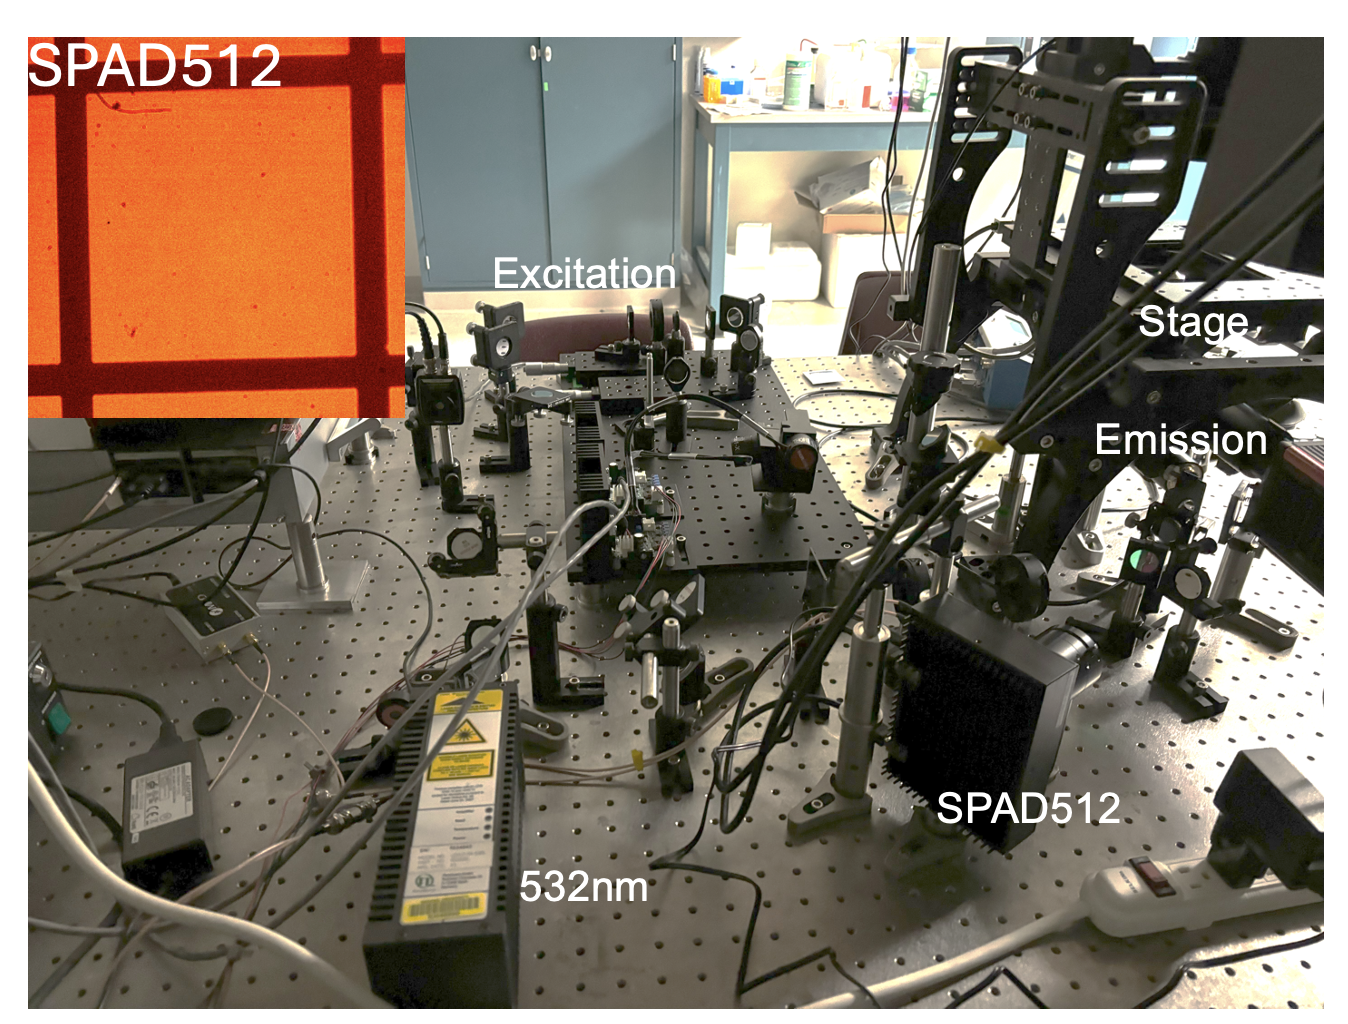
\includegraphics[width=14cm]{/Users/cwseitz/git/cwseitz.github.io/docs/phd/spad/spad/media/SPAD512.png}
\caption{Experimental setup for widefield photon counting. A 532nm pulsed laser is directed through a spatial filter, galvo mirror, and passed through filtering and focusing optics to a 100X oil-immersion objective. Emission light of a 50um grid is projected onto the SPAD512 camera (inset)}
\end{figure*}    


In this study, we present a method for widefield single photon counting in order to rigorously count fluorophores in the sample and subsequently constrain single molecule localization. We investigate the theoretical properties of the zero-lag second-order coherence function $g^{(2)}(0)$ for widefield photon counting and its spatial properties. Using Bayesian analysis, we derive a posterior distribution on the number of active fluorescent emitters in a region of interest. We then combined this with single molecule localization algorithms and demonstrate resolution of multiple emitters using a multi-emitter fitting algorithm and report localization errors with respect to the Cramer-Rao bound.

\section{Basic Scheme}

\begin{figure*}[t]
\centering
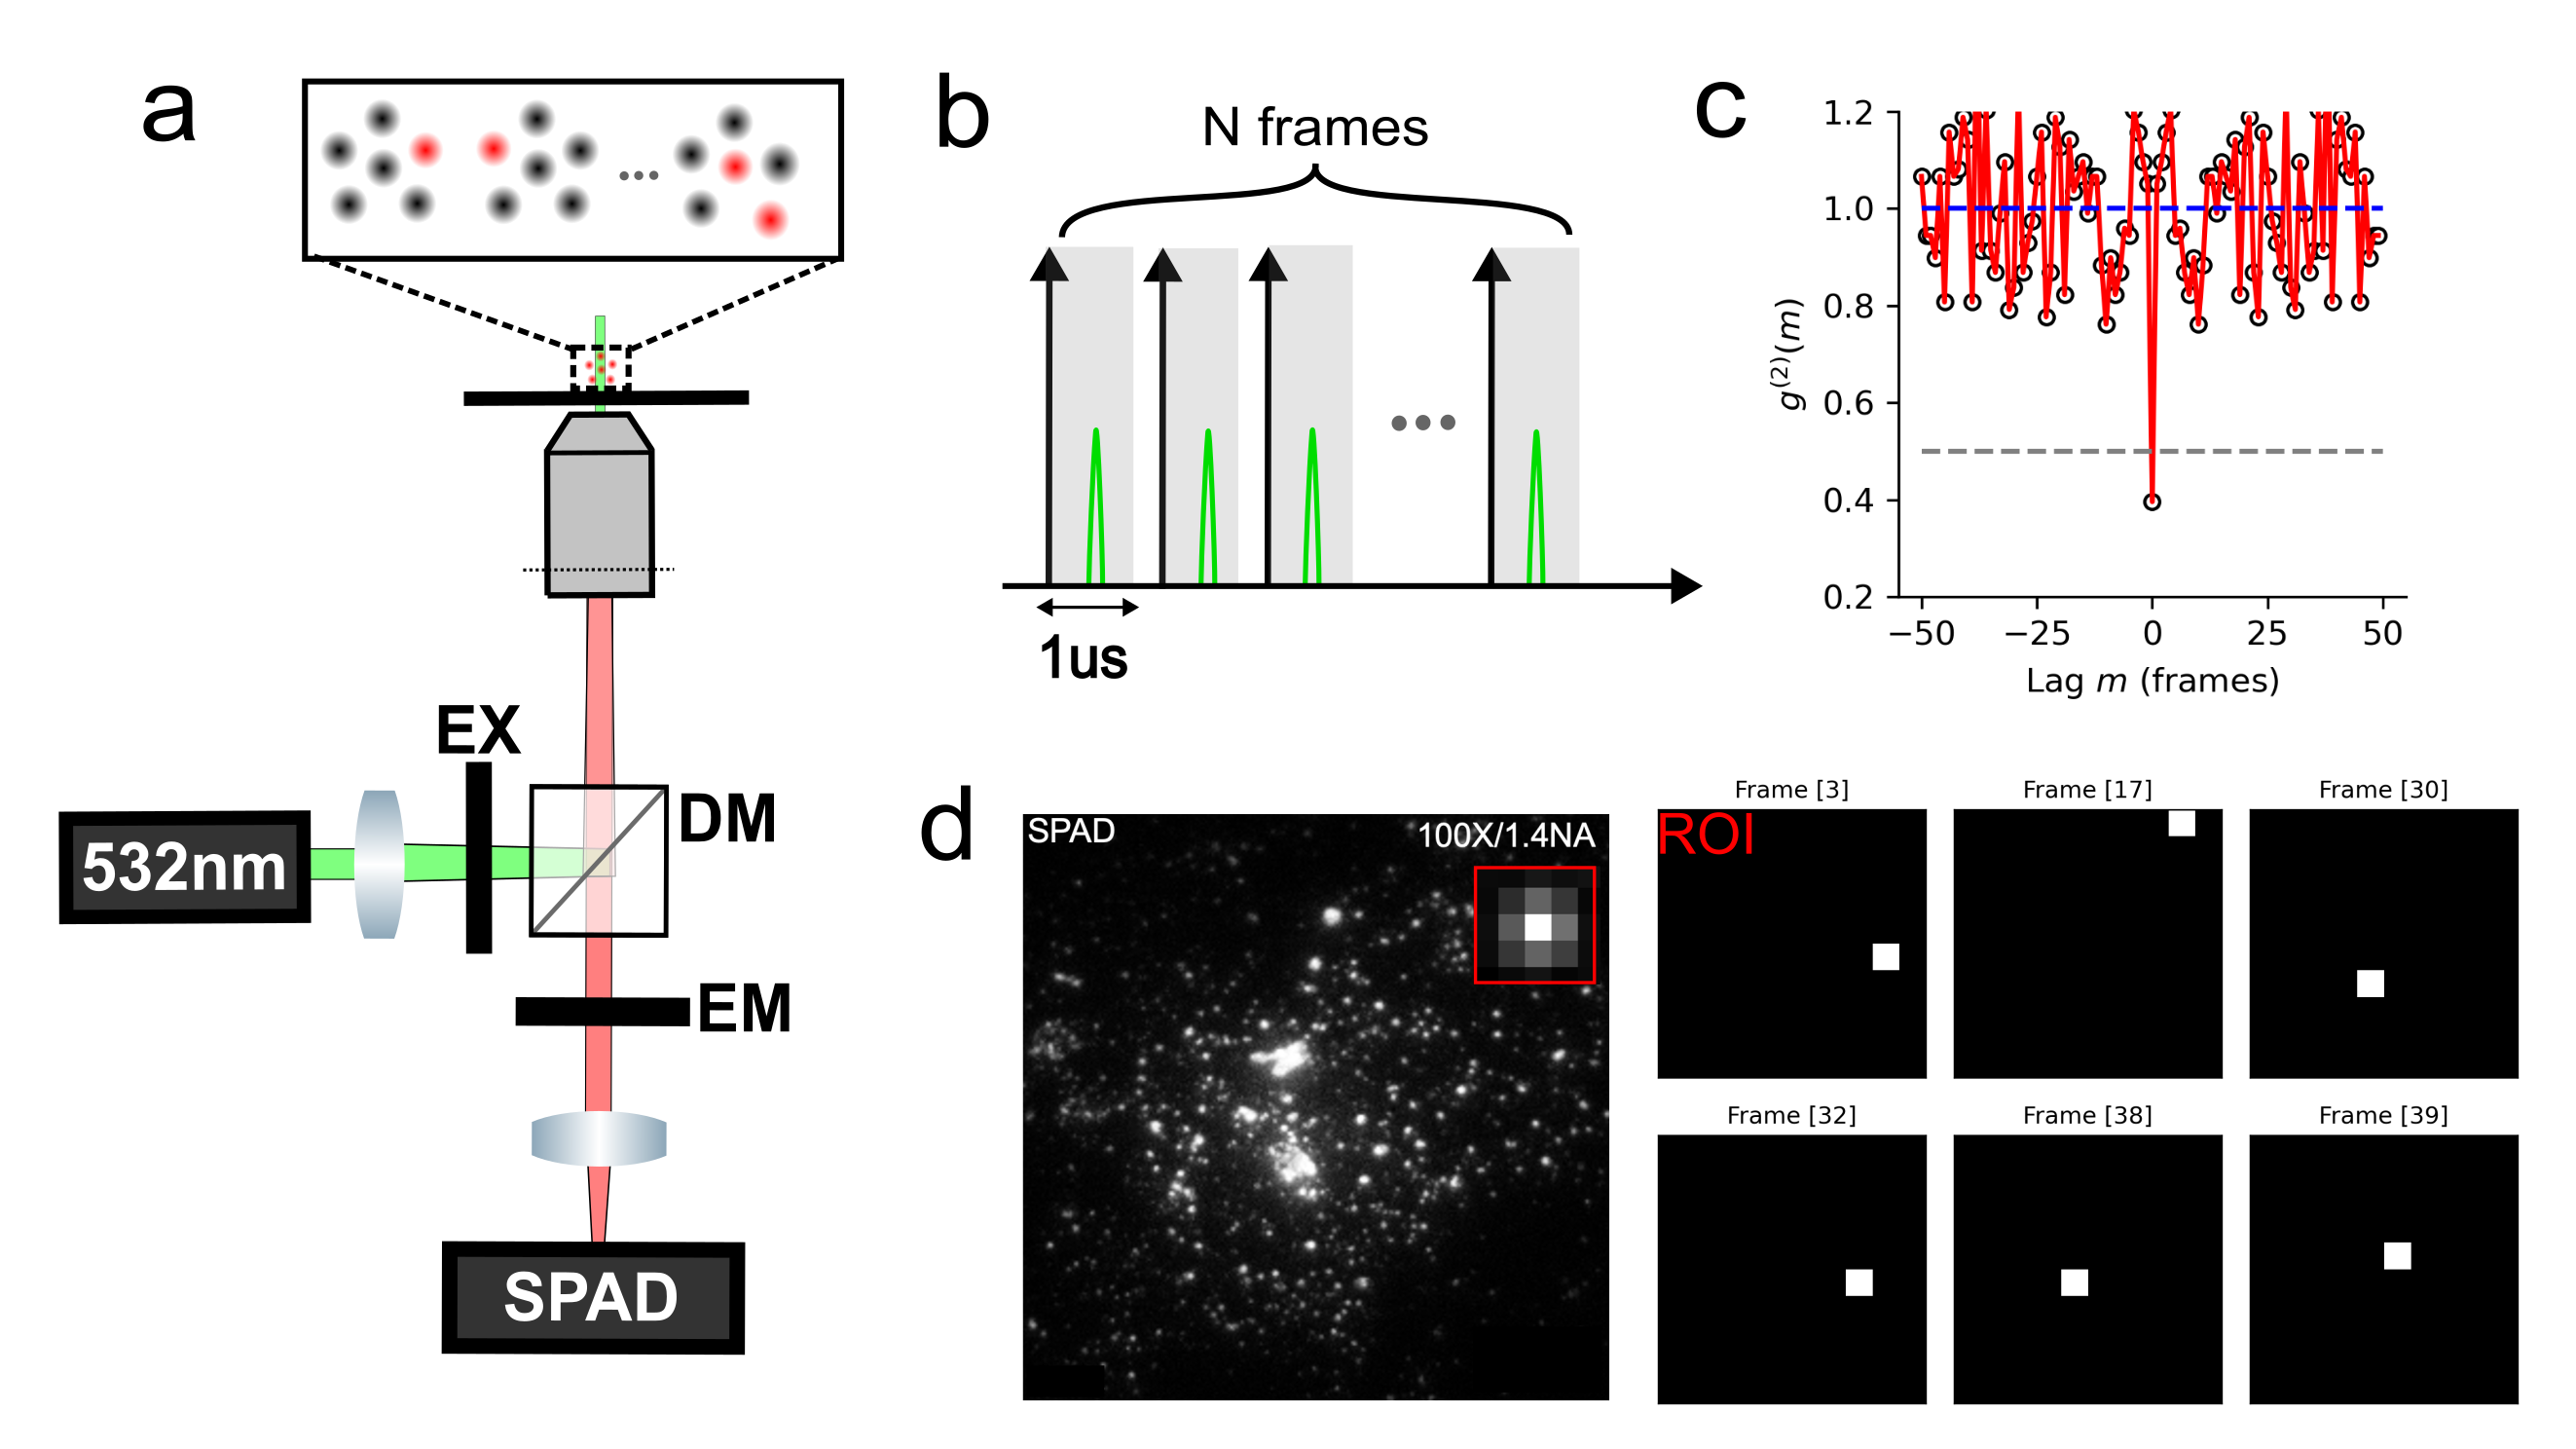
\includegraphics[width=14cm]{/Users/cwseitz/git/cwseitz.github.io/docs/phd/spad/spad/media/Figure-0.png}
\caption{Single photon counting with a SPAD array (a) Conventional widefield microscopy with integrated SPAD array (b) Single photon imaging scheme using 1us exposures containing a picosecond laser pulse (c) Sum of photon counts over a 5x5 region of interest (ROI), taken with $N_{\mathrm{frames}}=5\times 10^{5}$}
\end{figure*}    

We consider a simplified description of widefield photon counting for a a single photon source in the object plane labeled by a continuous-valued coordinate $\theta=(x_0,y_0)$. The spatial profile $O$ of the field in image space is presumed to have a Gaussian shape \parencite{Zhang2007,Richards1959,Gibson1989}.

\begin{equation}
O(x,y) = \frac{1}{2\pi\sigma^{2}}e^{-\frac{(x-x_{0})^2+(y-y_{0})^2}{2\sigma^2}}
\end{equation}

Therefore the field operator in object space is $\hat{E} \propto \hat{a}$ and in image space $\hat{E} \propto O(x,y)\hat{a}$. Since our SPAD detectors at the image plane must be discrete, the total field at a detector element $k$ centered in image space at $s_k=(u_k,v_k)$ is then given by integrating over pixels of width $\delta$. Moreover, the Gaussian $O$ is presumed to be isotropic and therefore we have $\hat{E}(s_k) \propto \Gamma_{x}(u_k,x_{0})\Gamma_{y}(v_k,y_0)$. For example,

\begin{align*}
\Gamma_{x}(u_k,x_{0}) &= \\ \frac{1}{\sqrt{2}}\left(\mathrm{erf}\left(\frac{u_k+\frac{1}{2}-x_{0}}{\sqrt{2}\sigma}\right) -\mathrm{erf}\left(\frac{u_k-\frac{1}{2}-x_0}{\sqrt{2}\sigma}\right)\right)
\end{align*}

We now consider the case of pulsed excitation where the interval between pulses much longer than the fluorescence lifetime. Upon excitation of an isolated fluorescent emitter, a photon is detected at a particular detector element $k$ with probability $\zeta_k \propto \langle \hat{E}^{\dagger}(s_k)\hat{E}(s_k)\rangle = \frac{1}{2}\Gamma_{x}^2 \Gamma_{y}^2\mathrm{Tr}(\rho a^{\dagger}a)$ where $\rho$ is the density matrix for a two-level system. Similarly, the probability of detection in a region of interest collecting all photons emitted is $\zeta\propto \mathrm{Tr}(\rho a^{\dagger}a)$. Here, we are primarily concerned with the latter quantity, and its application in counting fluorescent emitters.

\begin{figure*}[t]
\centering
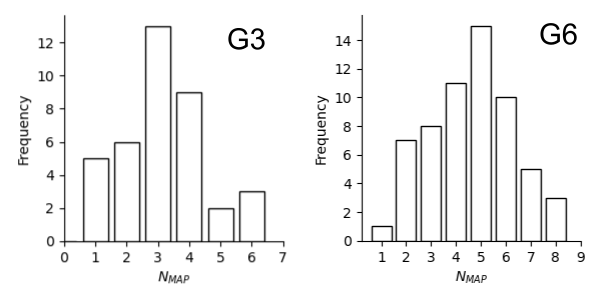
\includegraphics[width=12cm]{/Users/cwseitz/git/cwseitz.github.io/docs/phd/spad/spad/media/Figure-5.png}
\caption{Single and multi-emitter localization error on sums of photon counts. (left) Localization uncertainty for simulated data for different values of $N$, plotted with respect to the Cramer-Rao lower bound, shown in dashed gray. (right) Multi-emitter localization by MCMC sampling for $N=3$, colors indicate a cluster of samples i.e., a single localization. All data was generated with a background rate $\langle \bold{n}_{\mathrm{background}} \rangle = \lambda N_{\mathrm{frames}}/d^{2}$ per pixel. Scalebar 360nm}
\end{figure*}   

By temporarily ignoring the spatial profile described by (1), we derive a likelihood on the number of fluorophores in a small ROI with a lateral dimension $d = 5$ pixels. For $N$ fluorophores emitting photons which can be detected within a ROI of the SPAD array, the number of signal photons measured $n_{\mathrm{signal}}$ following a single excitation pulse will have Binomial statistics $n_{\mathrm{signal}} \sim \mathrm{Binom}(N,\zeta)$. Photon pile-up at a single detector element can be safely neglected in this model due to its relatively low likelihood. We then model the background signal within the region of interest as a coherent state, which must follow Poissonian statistics $n_{\mathrm{background}} \sim \mathrm{Poisson}(\lambda)$ for an expected number $\lambda$ of background counts in the ROI per frame. The total number of counts $n=n_{\mathrm{signal}}+n_{\mathrm{background}}$ detected in the region of interest following a single pulse is then distributed by the likelihood

\begin{equation}
p(n=n' \mid N, \zeta) = \sum_{i=0}^{\infty} \binom{N}{i} \zeta^i (1-\zeta)^{N-i} \frac{\lambda^{n'-i}}{(n'-i)!} e^{-\lambda}
\end{equation}

The expression in (2) represents a convolution of Poisson and Binomial probability mass functions. This result is the primary means of inference of the number of active emitters $N$ in a ROI.

In order to begin to perform localization in non-sparse ROIs, we write a posterior distribution on the Binomial parameters used in the likelihood (2) using Bayes rule

\begin{equation}
p(N,\zeta\lvert x) \propto p(x\lvert N,\zeta)p(\zeta)
\end{equation}

We use a Gaussian prior on $\zeta$ i.e., $p(\zeta) = \mathcal{N}(\mu_{\zeta},\sigma_{\zeta})$ with $\mu_{\zeta}=0.01$ and $\sigma_{\zeta}=0.005$. Prior uncertainty in the value of $\zeta$ stems from fluorophores with potentially heterogeneous photophysical properties as well as varying laser power throughout the excited region. This posterior can be integrated over $\zeta$ to produce a posterior distribution on the fluorophore number $N$ i.e., $p(N=N'\lvert n) \propto \int_{0}^{1} \prod_{j} p(n_{j}\lvert N',\zeta)p(\zeta) d\zeta$ which can be estimated using Monte Carlo methods. Monte Carlo integration is employed to integrate out $\zeta$. This involves sampling many $\zeta$ values from the Gaussian prior. For each sampled $\zeta$, the likelihood $(P(x\lvert\zeta_i)$ is computed, which, in this case, involves calculating the convolution of binomial and Poisson probability mass functions. These likelihood values are then weighted by the prior probabilities $P(\zeta)$. The final result is obtained by averaging these weighted likelihoods over all sampled $\zeta$, which approximates the integral:

\begin{equation*}
\int P(x\lvert\zeta) P(\zeta) \, d\zeta \approx \frac{1}{M} \sum_{i=1}^N P(x\lvert\zeta_i) P(\zeta_i)
\end{equation*}

where $M$ is the number of samples, $(P(x\lvert\zeta_i)$ is the likelihood of observing the data. This method provides a powerful way to handle the integration of complex or high-dimensional functions, especially when analytical solutions are intractable.


 The final posterior is then estimated by minibatching the data into batches of $10^3$ frames and averaging the posterior $p(N\lvert n)$ over minibatches. The fluorophore number $N$ within each ROI is then estimated by the maximum aposteriori (MAP) estimate $N^{*}$ given by this distribution.

For localization, we notice that (2) is well approximated by a Poisson distribution for a large frame number, making the localization procedure similar to conventional intensity-based methods \parencite{Smith2010}. Denoting the fluorophore coordinates by $\theta$ and vector of total counts in the region of interest $\bold{n}$, we have the following log-likelihood


\begin{align}
\ell(\bold{n}\lvert \theta) &= -\log \prod_{k} \frac{e^{-\left(\mu_{k}\right)}\left(\mu_{k}\right)^{\bold{n}_k}}{\bold{n}_k!}\\
&= \sum_{k}  \log \bold{n}_k! + \mu_{k} - \bold{n}_k\log\left(\mu_{k}\right)
\end{align}

\begin{figure}[t]
\centering
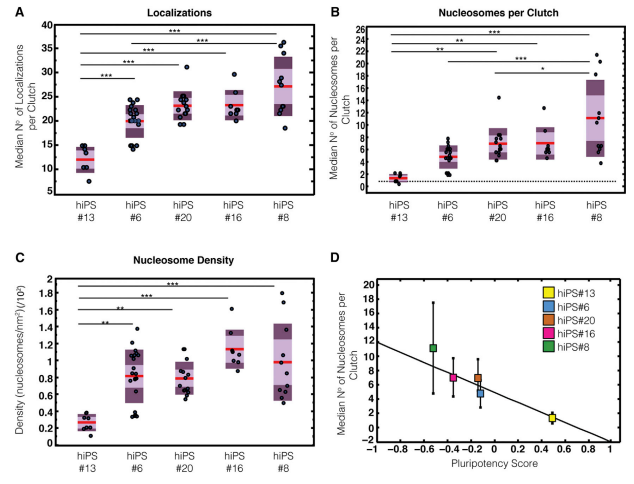
\includegraphics[width=12cm]{/Users/cwseitz/git/cwseitz.github.io/docs/phd/spad/spad/media/Figure-4.png}
\caption{Posteriors on the number of fluorescent emitters $N$ and localization for $N^{*}=1$ (left) and $N^{*}=2$ (right) quantum dots. Scalebars 360nm}
\end{figure}   

where, in the multi-emitter regime the expected photon count at a pixel is $\mu_{k} = \langle \bold{n}_k\rangle =\sum_{m=1}^{N^{*}} \mu_{k,m}$ given $\mu_{k,m}=\zeta N_{\mathrm{frames}}\Gamma_{x}(u_k,x_{0,m})\Gamma_{y}(v_k,y_{0,m}) + \lambda N_{\mathrm{frames}}/d^{2}$. In the multi-emitter regime, optimization of (4) by sampling is a suitable choice (see Results). 


\section{Results}

Quantum dots coated on a glass coverslip were excited using a picosecond $532\mathrm{nm}$ pulsed laser triggered at $500\mathrm{kHz}$. Emission light was collected using an oil-immersion 100$\times$ objective with numerical aperture (NA) 1.4 (Nikon). The emission signal was then filtered to exclude the laser line (Semrock) and projected onto the SPAD512 sensor (Pi Imaging Technologies) using a tube lens. A simplified diagram of the complete system is depicted in (Figure 1a). Each acquisition consists of $N=5\times 10^{5}$ frames (500ms), synchronized with each laser pulse, using a $1\mathrm{us}$ exposure per frame (Figure 1b,d). To confirm the presence of single photon sources in the sample, we investigated properties of the zero-lag second order coherence function $g^{(2)}(0)$. The following empirical estimate of $g^{(2)}(0)$ is used \parencite{Israel2017}

\begin{equation}
g^{(2)}(0) = \frac{G^{(2)}(0)-B}{\langle G^{(2)}(m\neq 0)\rangle -B}
\end{equation}

where $B = N_{\mathrm{frames}}\lambda\zeta$ is the expected number of background-signal coincidences in the region of interest. The quantity $G^{(2)}(m)$ represents the number of signal-signal coincidences in the region of interest at a lag time $m$. The quantity $\langle G^{(2)}(m\neq 0)\rangle$ is the average number of coincidences in pairs of frames at nonzero lag $m \in [1,100]$, in units of frames. As expected, simulation from the likelihood (2) shows saturation of $g^{(2)}(0)$  with increasing values of $N$ (Figure 1c). Moreover, bright clusters of quantum dots exhibit elevated $g^{(2)}(0)$ values as can be seen in maps of the $g^{(2)}(0)$ computing using sliding window over the array (Figure 1e).

For localization by optimization of (4), we use Goodman and Weare's Markov Chain Monte Carlo (MCMC) algorithm \parencite{Goodman2010} to sample from the posterior on fluorophore locations. In all simulations we assume a uniform prior on coordinates over the ROI and $\zeta$ is known and identical over fluorophores. Fluorophore locations can then be estimated from the posterior samples by K-means clustering of the $(x,y)$ coordinates of the first particle and identification of cluster centers (Figure 2a). To validate our estimator, we compare its RMSE to the single emitter Cramer-Rao lower bound, which bounds the variance of a statistical estimator of $\theta$, from below (Chao 2016). For an isolated emitter, the Poisson log-likelihood (5) is convenient for computing the Fisher information matrix for $\theta$ and thus the The Fisher information is \parencite{Smith2010}

\begin{figure}[t]
\centering
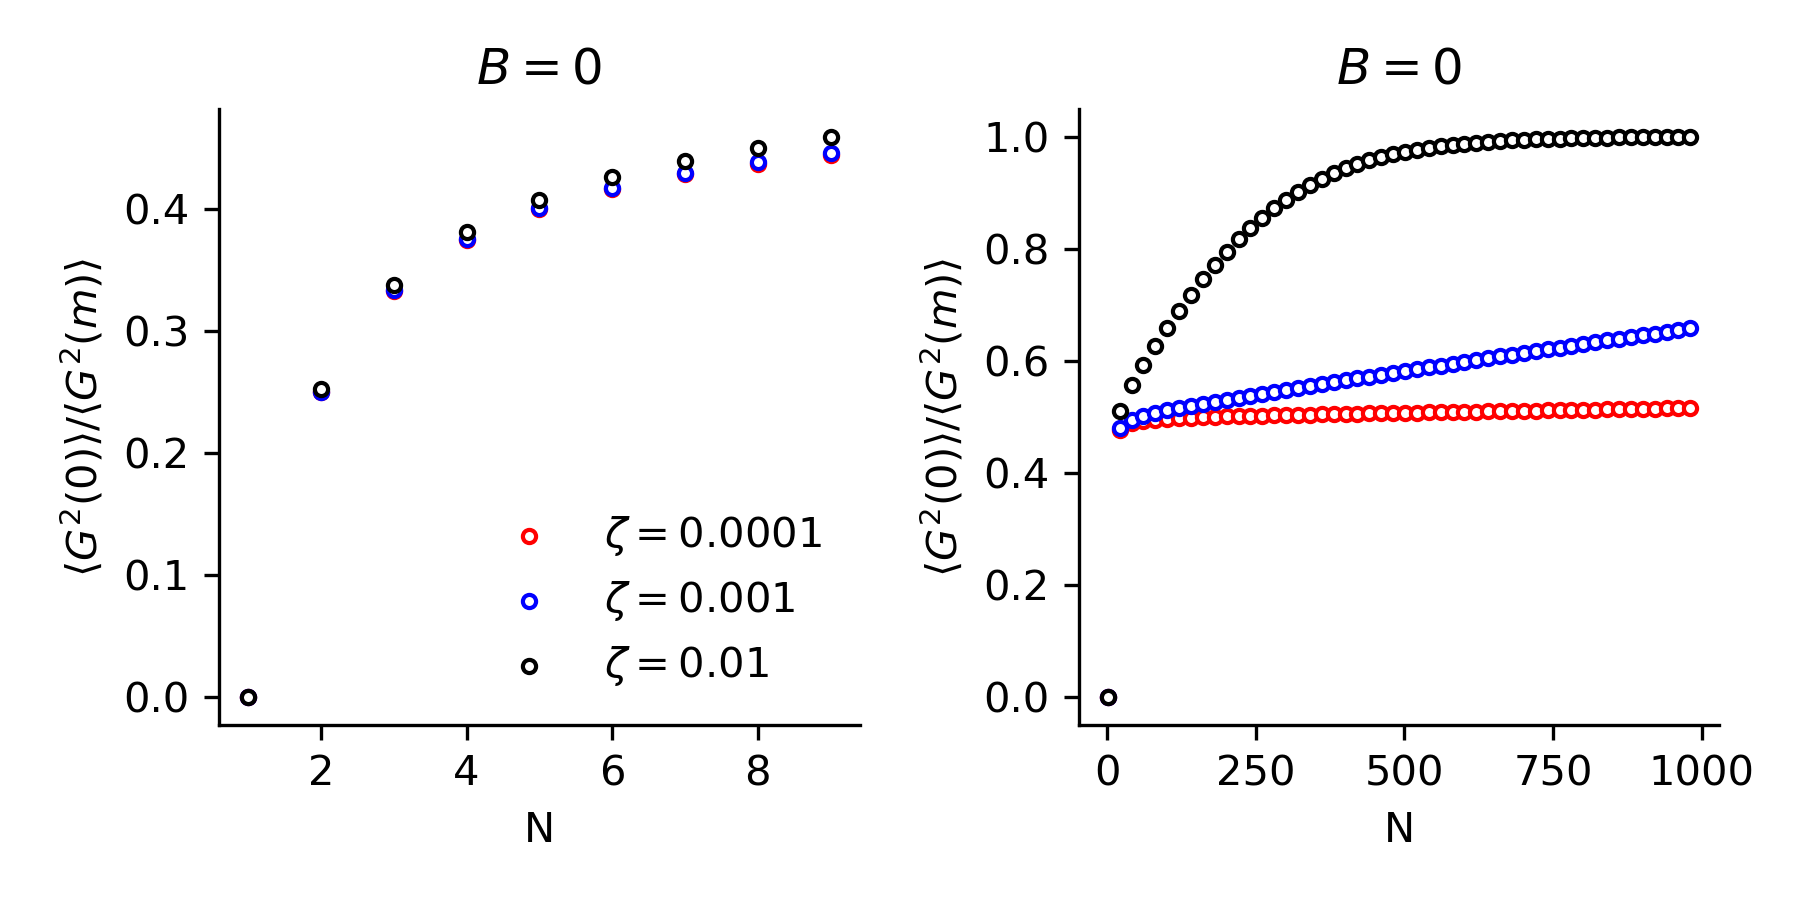
\includegraphics[width=12cm]{/Users/cwseitz/git/cwseitz.github.io/docs/phd/spad/spad/media/g20g2m.png}
\caption{Scaling of $g^{(2)}(0)$ under zero background conditions. (left) Scaling of $g^{(2)}(0)$ for small $N$. (right) Scaling of $g^{(2)}(0)$ for large $N$}
\end{figure}   

\begin{equation}
I_{ij}(\theta) = \sum_{k}\frac{1}{\mu_{k}}\frac{\partial \mu_{k}}{\partial\theta_{i}}\frac{\partial \mu_{k}}{\partial\theta_{j}}
\end{equation}

The Cramer-Rao bound is then found by $\mathrm{var}(\theta) \geq I^{-1}(\theta)$. We find that for thousands of expected signal photon counts, localization uncertainty lies in an acceptable range for localization microscopy (Figure 2b). Example posteriors and multi-emitter fitting on experimental quantum dot data are found in (Figure 3). The $\zeta$ value is treated as unknown but homogeneous across fluorophores in the ROI. \textit{A major criticism is likely that we have not measured $\zeta$ precisely and that we can only provide self-consistency for its simultaenous value with $N$}.

Averaging $G^{(2)}(0)$ over many realizations (sequences of $N_{\mathrm{frames}}$), gives the expected value $\langle G^{(2)}(0)\rangle $

\begin{equation}
\langle G^{(2)}(0)\rangle = N_{\mathrm{frames}}(1 - (1-\zeta)^n - n\zeta (1-\zeta)^{n-1})
\end{equation}

Since $G^{(2)}(m)$ is already averaged over $m$, $\langle G^{(2)}(m) $ is effectively a constant over realizations, and must be

\begin{equation}
\langle G^{(2)}(m)\rangle =  N_{\mathrm{frames}} \left(1 - \left((1-\zeta)^n\right)\right)^2
\end{equation}

Ignoring the effect of background signal $\langle g^{(2)}(0)\rangle =\langle G^{(2)}(0)\rangle/\langle G^{(2)}(m)\rangle$, which rapidly approaches $1/2$ as a function of $N$, and then saturates and very slowly approaches its maximum value of 1. This is consistent with the idea that for very large number of active fluorescent emitters, the statistics should become Poisson.


\begin{figure*}[t]
\centering
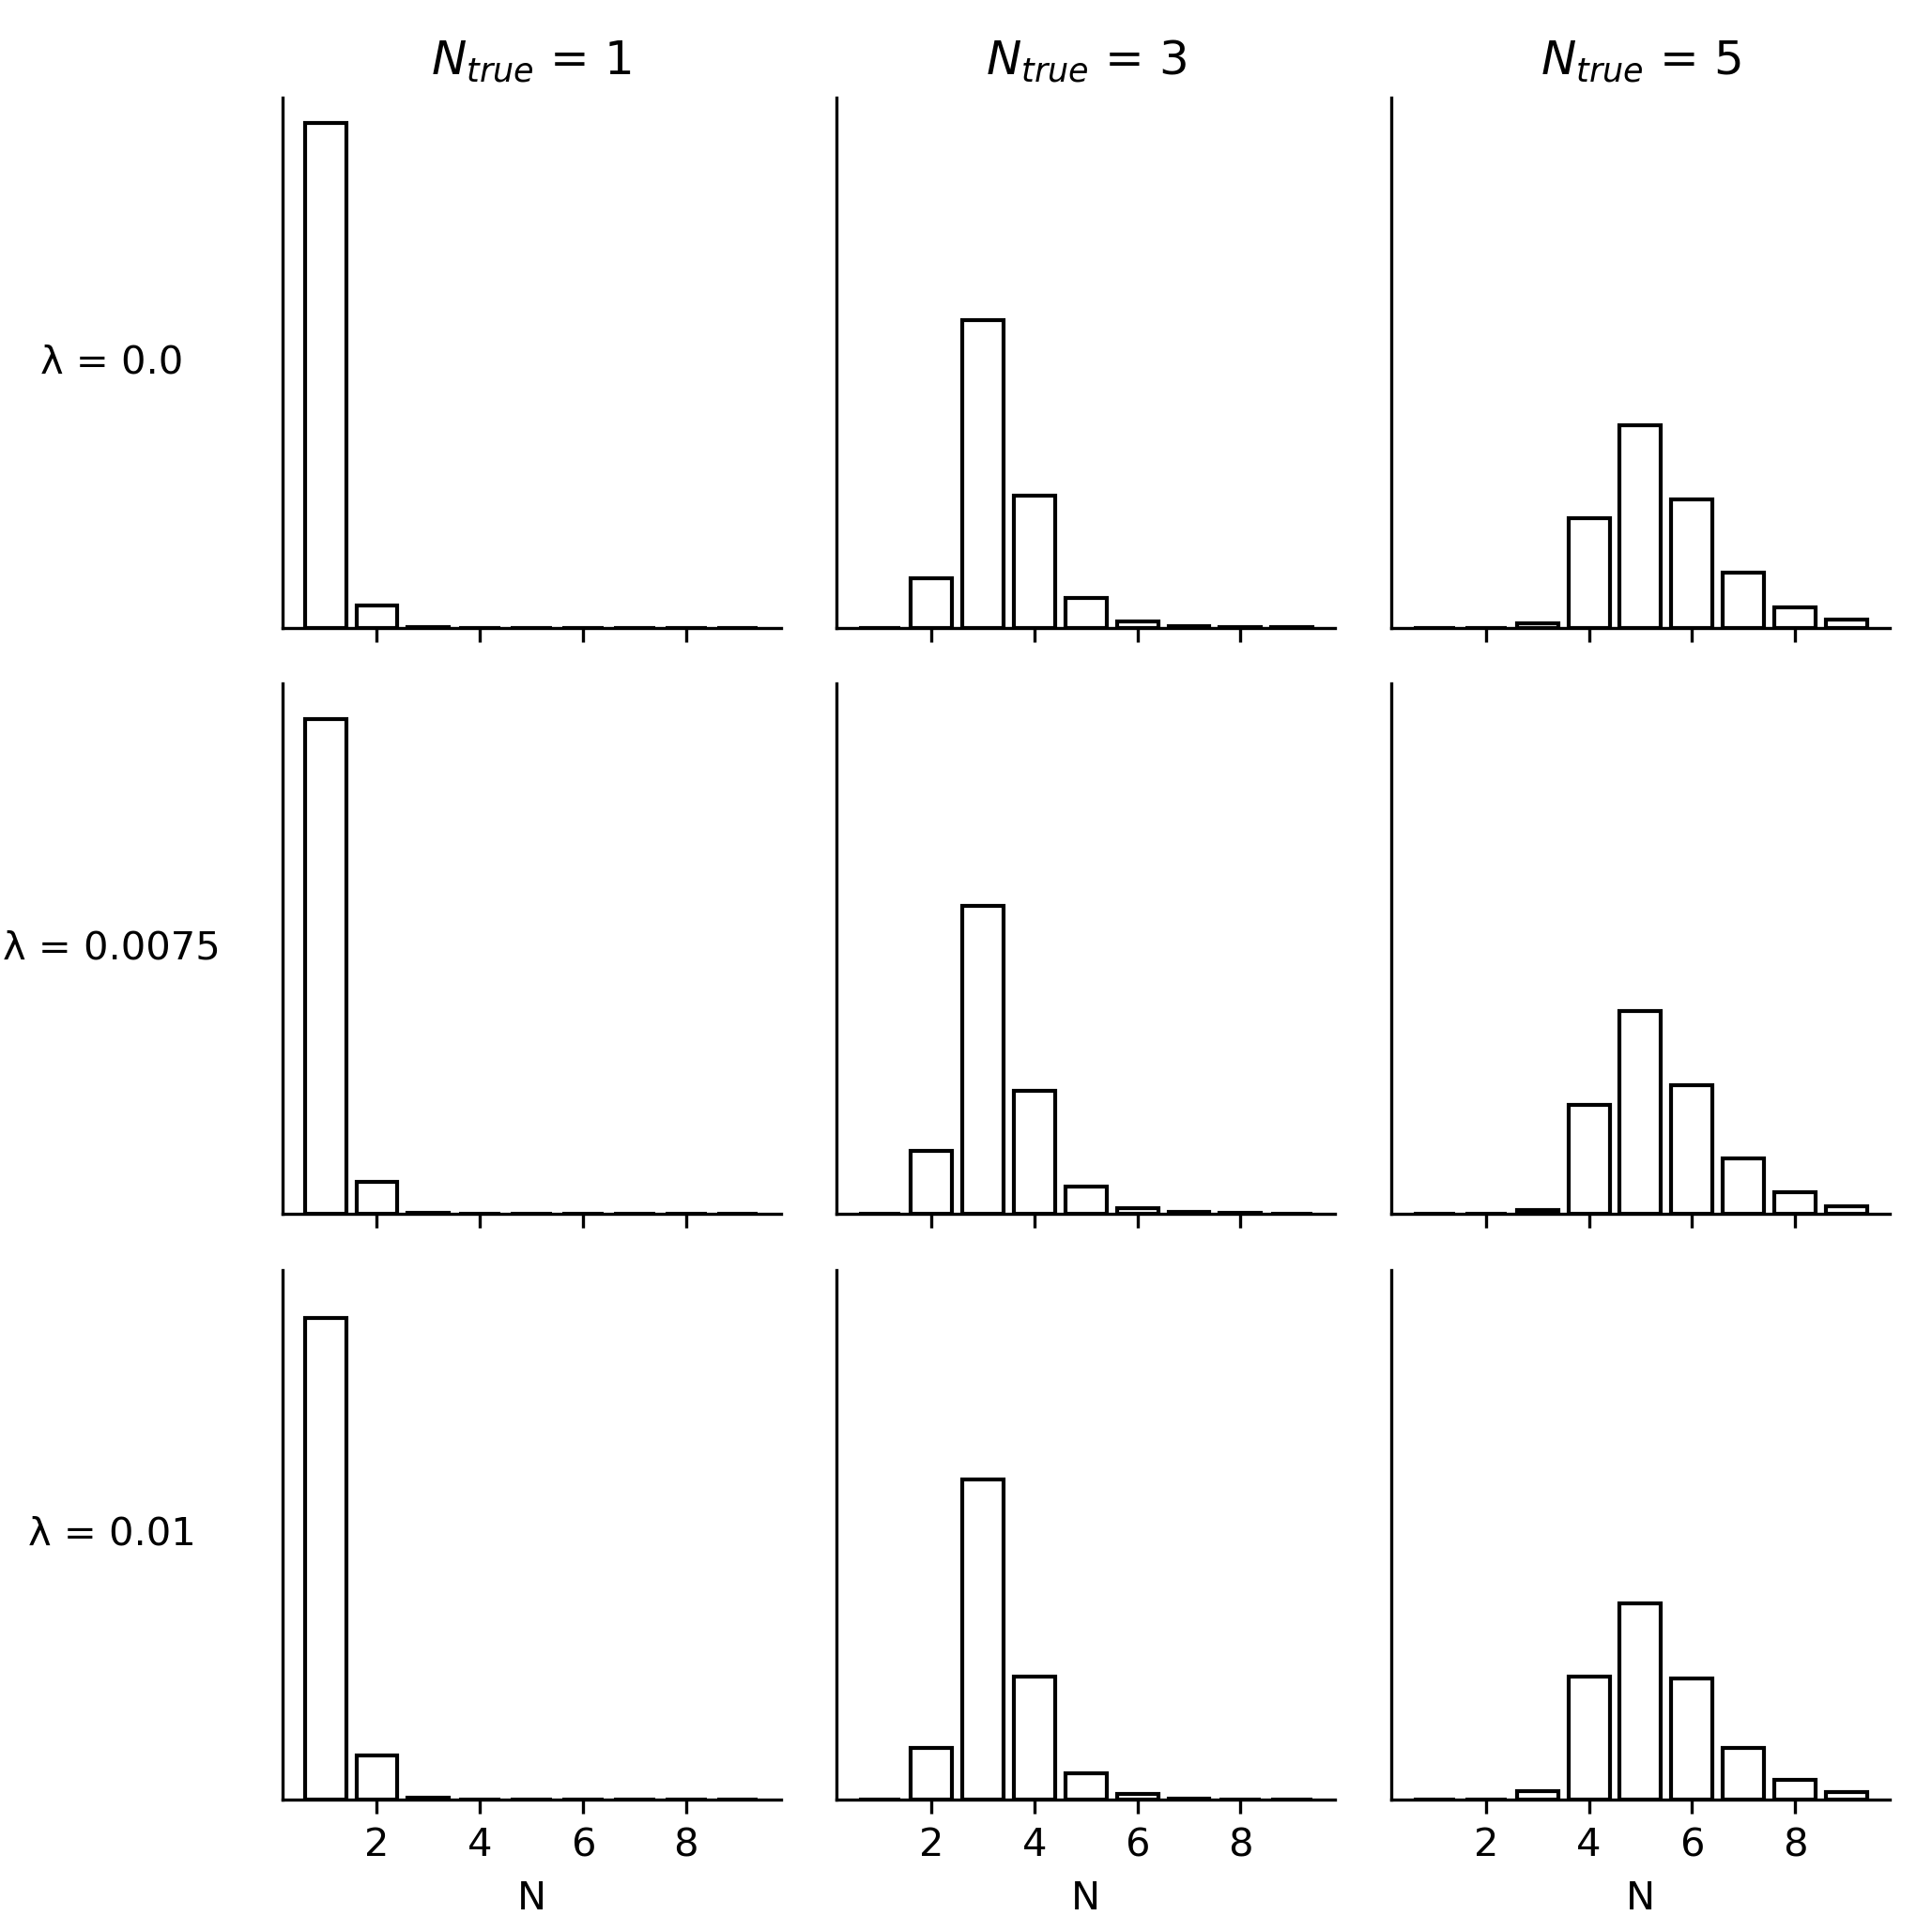
\includegraphics[width=14cm]{/Users/cwseitz/git/cwseitz.github.io/docs/phd/spad/spad/media/PoissonBinomialPost-1.png}
\caption{Posterior distributions of the fluorophore number. Samples from the Poisson-Binomial convolution distribution using $\zeta=0.01$ for various values of $\lambda$ and $N=1,3,5$ were simulated. The variable $\zeta$ was integrated out by Monte Carlo integration, sampling 1000 $\zeta$ values from the posterior distribution (see main text for details)}
\end{figure*}    

\begin{figure*}[t]
\centering
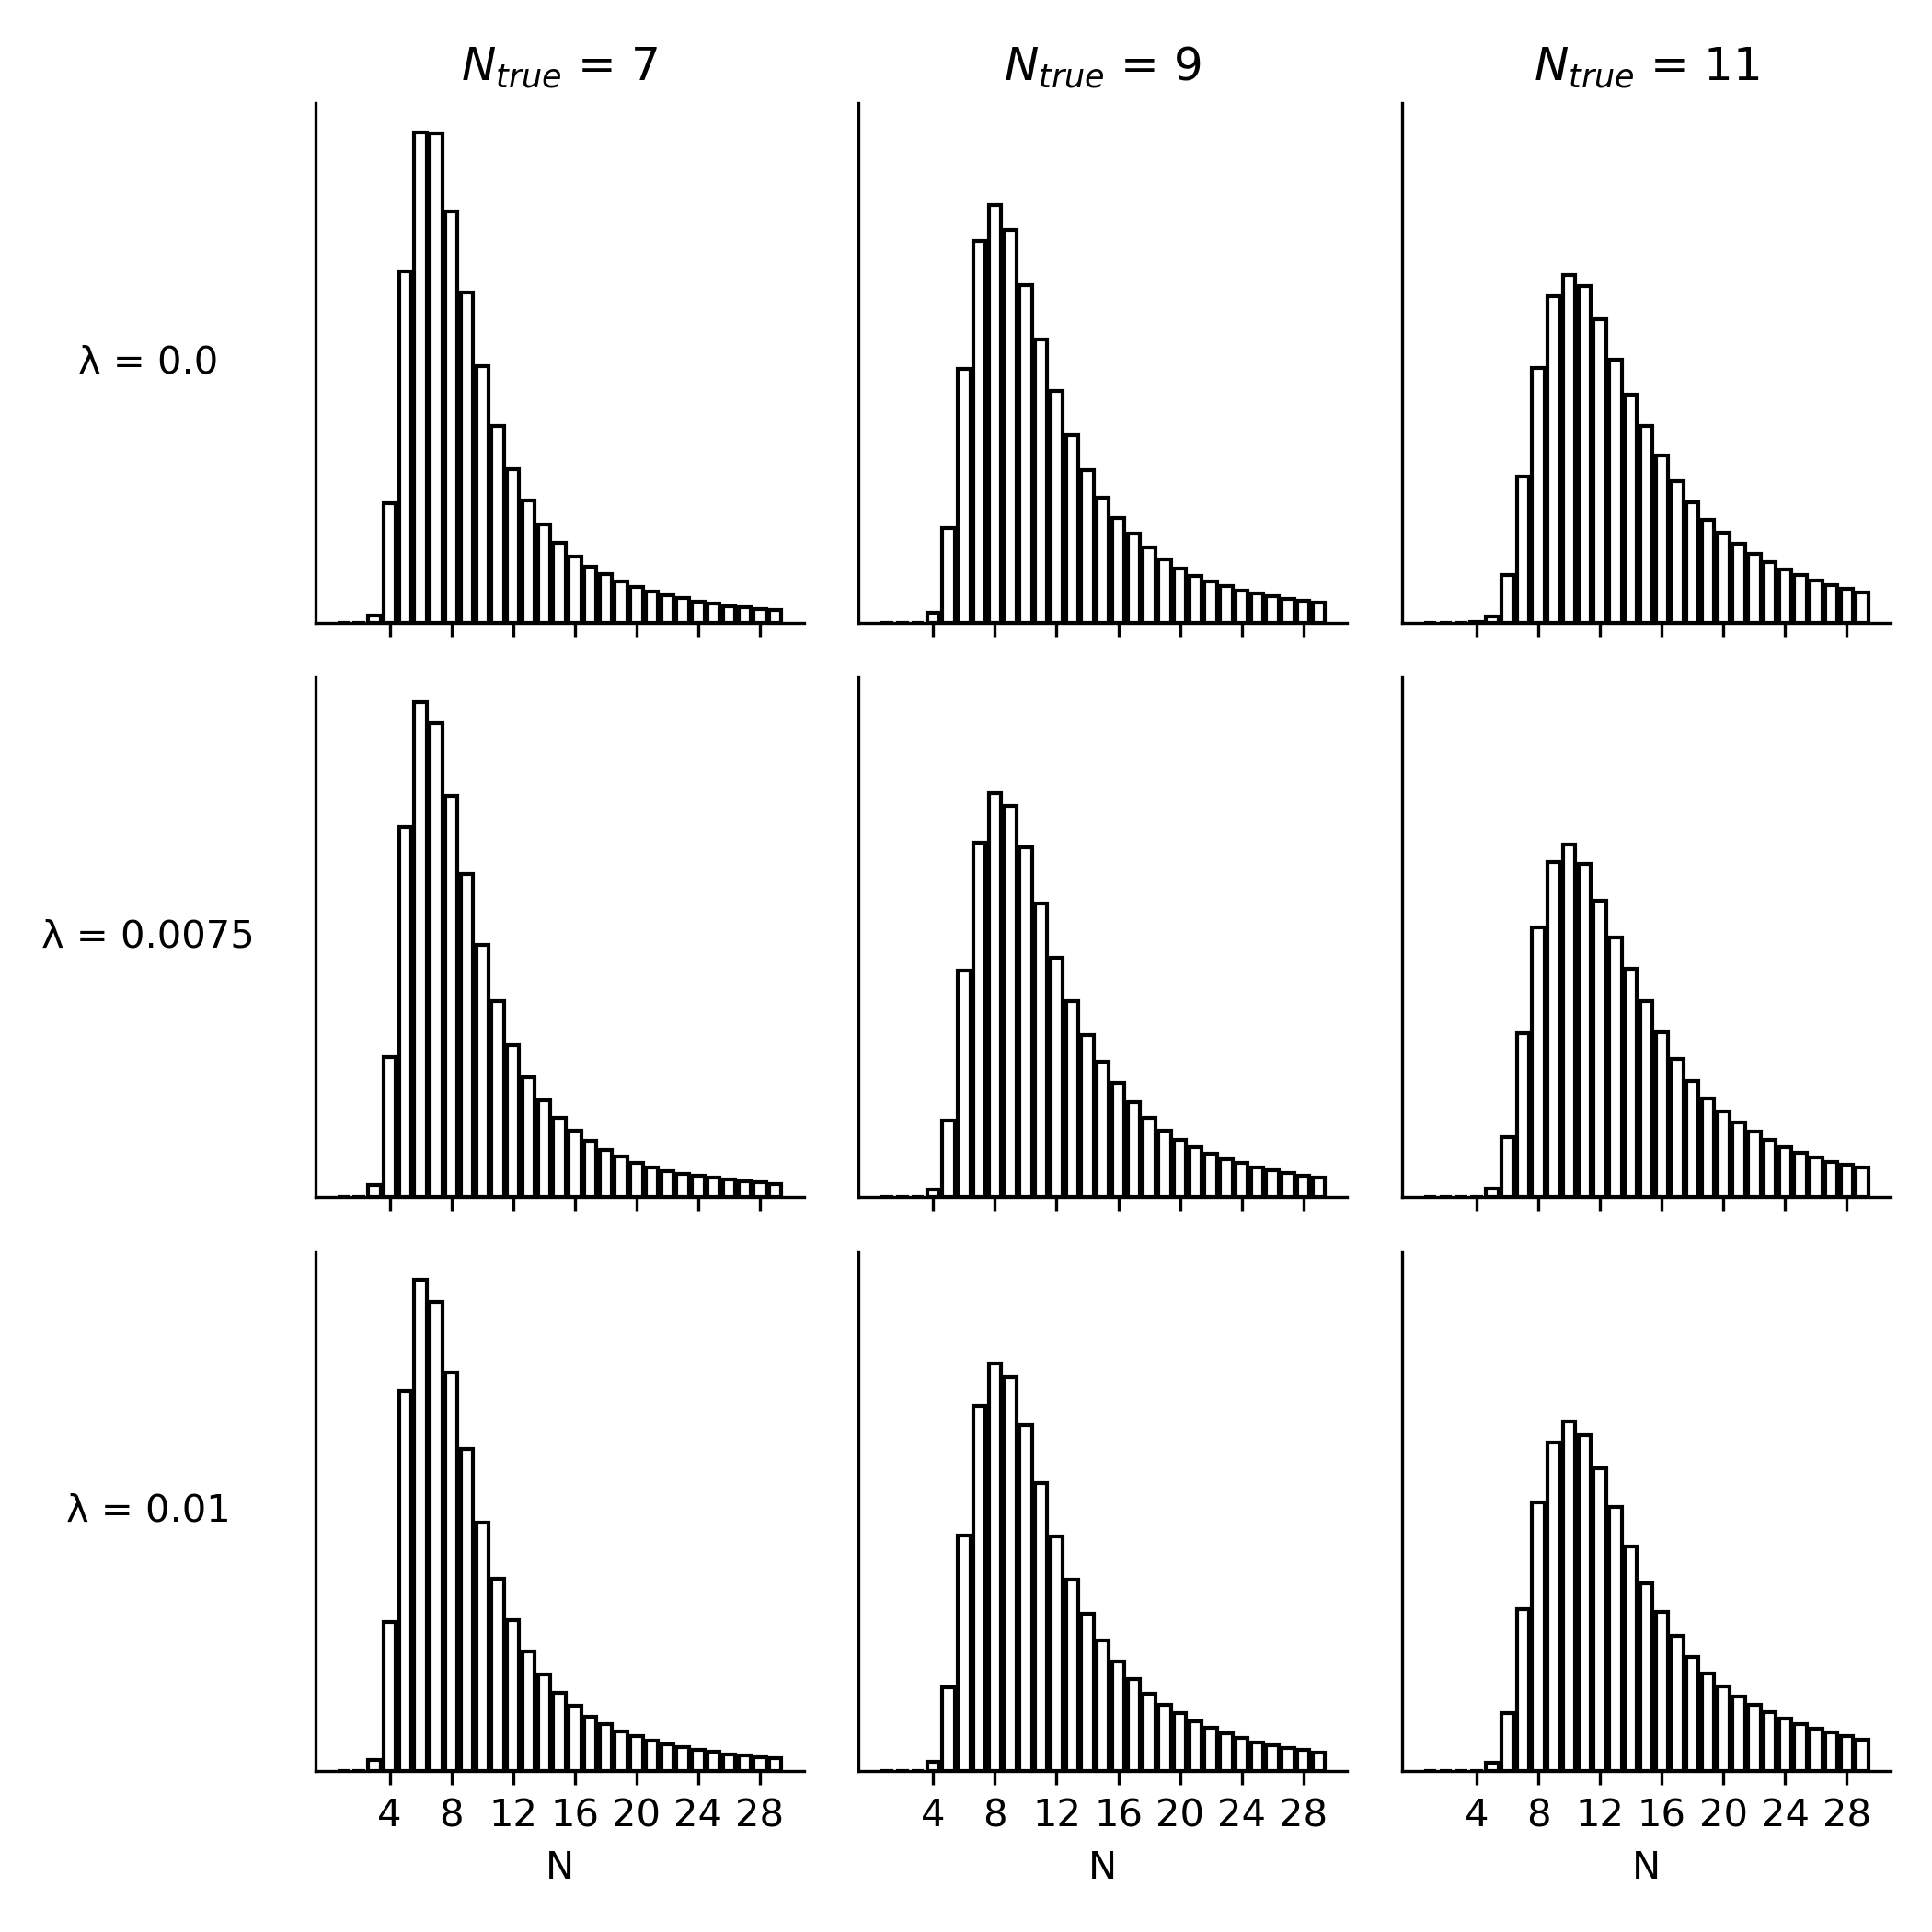
\includegraphics[width=14cm]{/Users/cwseitz/git/cwseitz.github.io/docs/phd/spad/spad/media/PoissonBinomialPost-2.png}
\caption{Posterior distributions of the fluorophore number. Samples from the Poisson-Binomial convolution distribution using $\zeta=0.01$ for various values of $\lambda$ and $N=7,9,11$ were simulated. The variable $\zeta$ was integrated out by Monte Carlo integration, sampling 1000 $\zeta$ values from the posterior distribution (see main text for details)}
\end{figure*}    



\section{Discussion}

Many fluorescent emitters exhibit random variations of brightness known as blinking. Blinking increases the observed photon-number fluctuations and could be expected to affect the value of $g^{(2)}(0)$ or the posterior on the number of active fluorescent emitters. However, the signal photon number per frame will follow Binomial statistics even in the presence of blinking, the only consequence of which is an effective reduction of the detection probability $\zeta$. If the effect of censoring photons by blinking and lowering the quantum yield can be accounted for, the technique used here may be compatible with common super-resolution techniques such as stochastic optical reconstruction microscopy (STORM). 

The acquisition times necessary to obtain sufficient photon counts for computing the necessary statistics can potentially be very short. Most fluorophores have relaxation times in the nanosecond range and thus photons can be collected at a rate of at tens of millions of excitation pulses per second. These rates are currently difficult to obtain, however, due to limitations in detector throughput. The SPAD camera used in this study has a minimum exposure time in the microsecond range. Furthermore, the data volume can quickly become intractable due to the need for several thousands of frames for a millisecond-scale exposure time. This is currently a complication for techniques like STORM and advancements in the automation for data acquisitions are necessary. The speed of MCMC based localization remains a limitation for post-processing, and optimization of the processing time for localization is left for future work. 

In conclusion, we propose a single molecule imaging technique that allows for simultaneous counting of localization of fluorescent molecules by modeling the quantum properties of fluorescence emission. The technique does not require a nonclassical light source and is designed to supplement standard single molecule localization microscopy techniques. The proposed method can be implemented with a standard widefield fluorescence microscope.


